\hypertarget{Classes_8c}{
\section{Classes.c File Reference}
\label{Classes_8c}\index{Classes.c@{Classes.c}}
}
{\tt \#include \char`\"{}CI\_\-common.h\char`\"{}}\par


Include dependency graph for Classes.c:\begin{figure}[H]
\begin{center}
\leavevmode
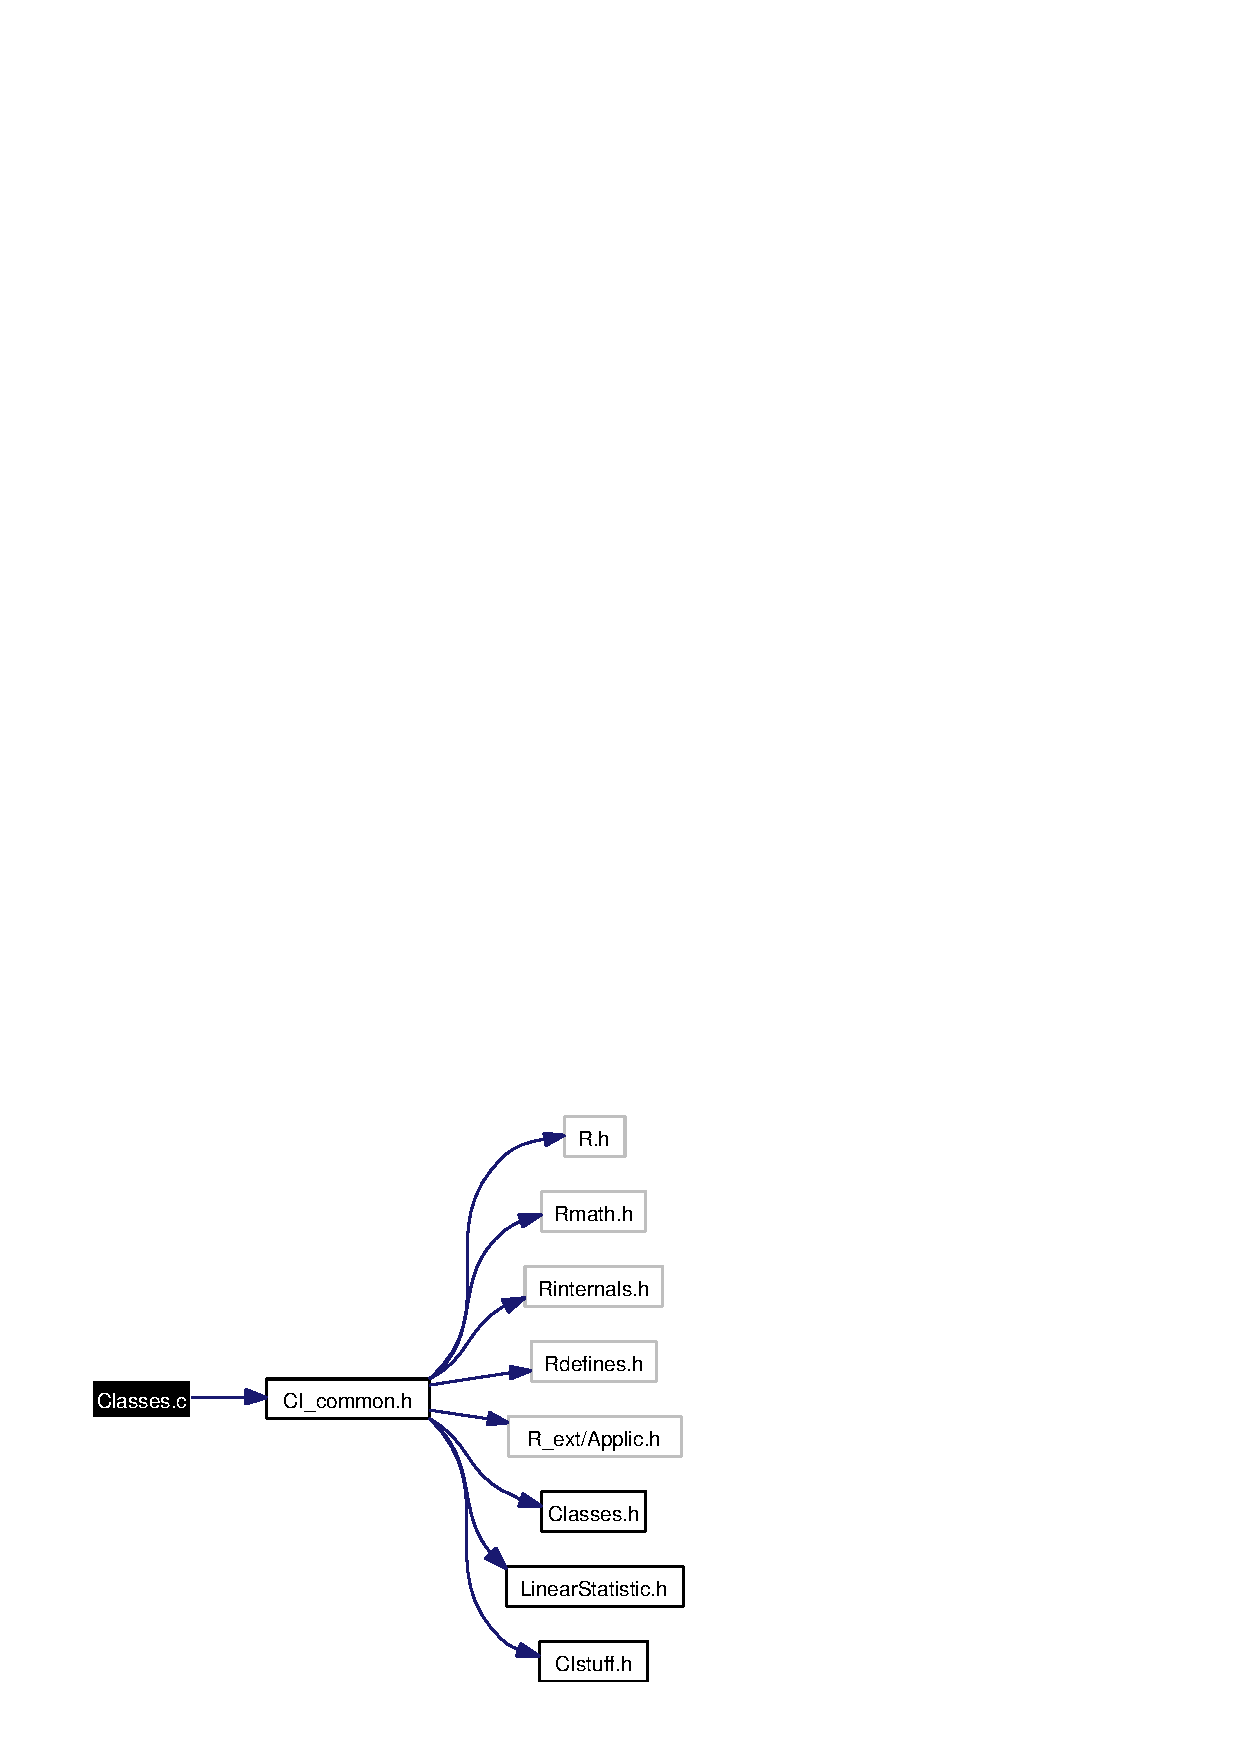
\includegraphics[width=168pt]{Classes_8c__incl}
\end{center}
\end{figure}
\subsection*{Functions}
\begin{CompactItemize}
\item 
SEXP \hyperlink{Classes_8c_a3}{coin\_\-init} (void)
\end{CompactItemize}
\subsection*{Variables}
\begin{CompactItemize}
\item 
SEXP \hyperlink{Classes_8c_a0}{CI\_\-expectation\-Sym}
\item 
SEXP \hyperlink{Classes_8c_a1}{CI\_\-covariance\-Sym}
\item 
SEXP \hyperlink{Classes_8c_a2}{CI\_\-sumweights\-Sym}
\end{CompactItemize}


\subsection{Detailed Description}
S4 classes

\begin{Desc}
\item[Author:]\begin{Desc}
\item[Author]hothorn \end{Desc}
\end{Desc}
\begin{Desc}
\item[Date:]\begin{Desc}
\item[Date]2005/07/28 15:04:29 \end{Desc}
\end{Desc}


Definition in file \hyperlink{Classes_8c-source}{Classes.c}.

\subsection{Function Documentation}
\hypertarget{Classes_8c_a3}{
\index{Classes.c@{Classes.c}!coin_init@{coin\_\-init}}
\index{coin_init@{coin\_\-init}!Classes.c@{Classes.c}}
\subsubsection[coin\_\-init]{\setlength{\rightskip}{0pt plus 5cm}SEXP coin\_\-init (void)}}
\label{Classes_8c_a3}




Definition at line 16 of file Classes.c.

References CI\_\-covariance\-Sym, CI\_\-expectation\-Sym, and CI\_\-sumweights\-Sym.

\subsection{Variable Documentation}
\hypertarget{Classes_8c_a1}{
\index{Classes.c@{Classes.c}!CI_covarianceSym@{CI\_\-covarianceSym}}
\index{CI_covarianceSym@{CI\_\-covarianceSym}!Classes.c@{Classes.c}}
\subsubsection[CI\_\-covarianceSym]{\setlength{\rightskip}{0pt plus 5cm}SEXP \hyperlink{Classes_8h_a1}{CI\_\-covariance\-Sym}}}
\label{Classes_8c_a1}




Definition at line 12 of file Classes.c.

Referenced by C\_\-Expect\-Covar\-Influence(), C\_\-Expect\-Covar\-Linear\-Statistic(), coin\_\-init(), R\_\-Expect\-Covar\-Influence(), and R\_\-Expect\-Covar\-Linear\-Statistic().\hypertarget{Classes_8c_a0}{
\index{Classes.c@{Classes.c}!CI_expectationSym@{CI\_\-expectationSym}}
\index{CI_expectationSym@{CI\_\-expectationSym}!Classes.c@{Classes.c}}
\subsubsection[CI\_\-expectationSym]{\setlength{\rightskip}{0pt plus 5cm}SEXP \hyperlink{Classes_8h_a0}{CI\_\-expectation\-Sym}}}
\label{Classes_8c_a0}




Definition at line 12 of file Classes.c.

Referenced by C\_\-Expect\-Covar\-Influence(), C\_\-Expect\-Covar\-Linear\-Statistic(), coin\_\-init(), R\_\-Expect\-Covar\-Influence(), and R\_\-Expect\-Covar\-Linear\-Statistic().\hypertarget{Classes_8c_a2}{
\index{Classes.c@{Classes.c}!CI_sumweightsSym@{CI\_\-sumweightsSym}}
\index{CI_sumweightsSym@{CI\_\-sumweightsSym}!Classes.c@{Classes.c}}
\subsubsection[CI\_\-sumweightsSym]{\setlength{\rightskip}{0pt plus 5cm}SEXP \hyperlink{Classes_8h_a2}{CI\_\-sumweights\-Sym}}}
\label{Classes_8c_a2}




Definition at line 12 of file Classes.c.

Referenced by C\_\-Expect\-Covar\-Influence(), C\_\-Expect\-Covar\-Linear\-Statistic(), coin\_\-init(), and R\_\-Expect\-Covar\-Influence().